\documentclass{article}

\usepackage{float}
\usepackage{graphicx}
\graphicspath{ {supporting info figures/} }
\usepackage[margin=1.5in]{geometry}

\usepackage[aboveskip=10pt,labelfont=bf,labelsep=period,justification=raggedright,singlelinecheck=off]{caption}
\renewcommand{\figurename}{Fig}

\title{Supporting Information}
\date{}

\begin{document}
\maketitle		

\renewcommand{\thefigure}{\Alph{figure}}

\section{Simulated Examples}
\subsection{Trefoil Plots}
For the trefoil example, the signal $Y$ consisted of a trefoil knot embedded in three dimensions containing 500 points. $Z + \epsilon$ was constructed by adding seven superfluous dimensions and isotropic Gaussian noise. Various degrees of noise were tested ($sd = 5, 10, 15, 20, 25, 30$). The first two plots depict Trustworthiness vs. Perplexity and the trustworthiness-maximizing embeddings for the $sd = 10$ case. The third plot shows the trustworthiness-maximizing perplexity for the different degrees of noise.

\begin{figure}[!h]
\centering
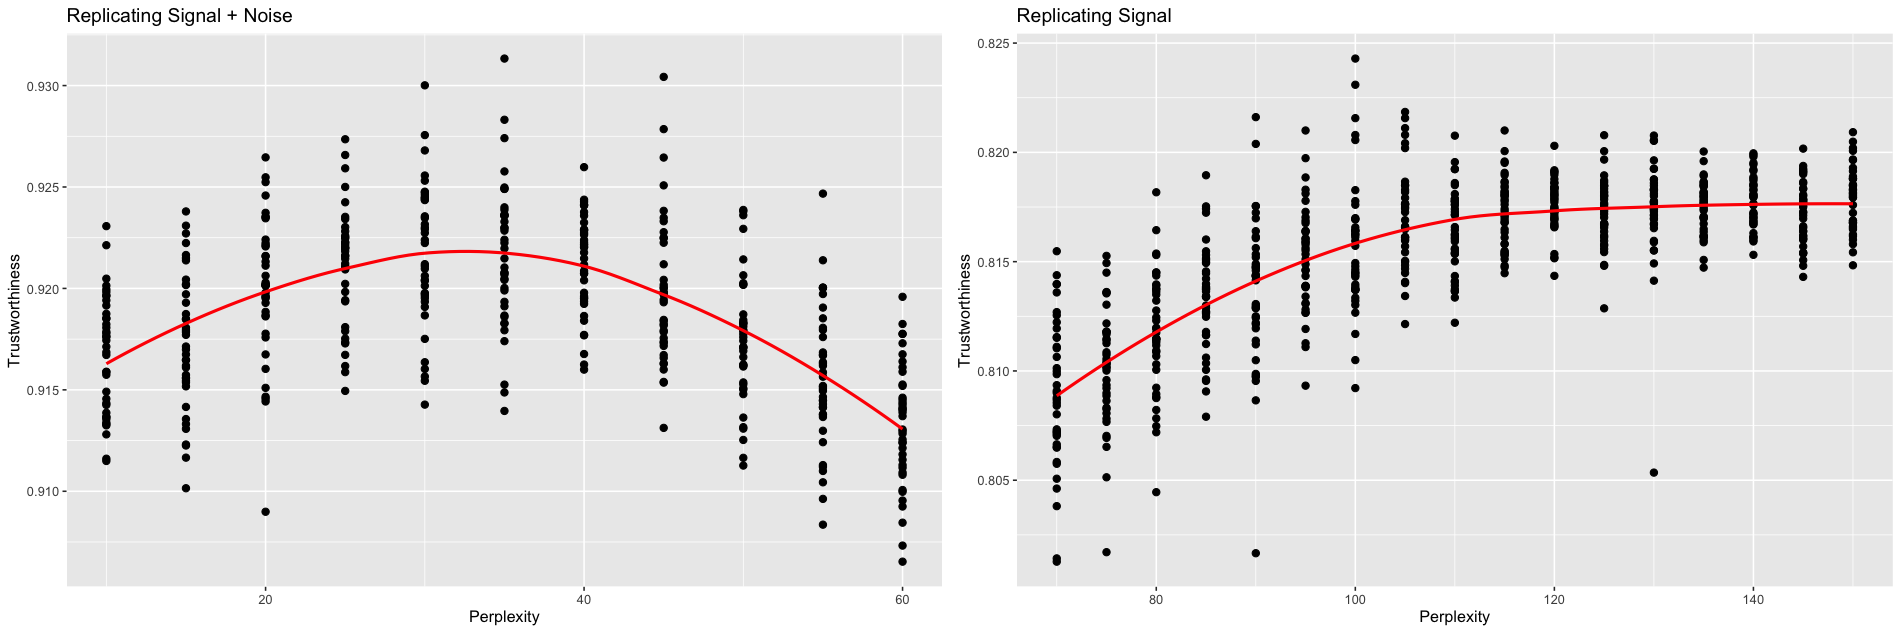
\includegraphics[scale=0.85]{Fig S1}
\caption{{\bf Trustworthiness vs. perplexity for sd = 10 (trefoil).}
t-SNE outputs were calculated with varying perplexities. Local performance was measured via trustworthiness. The trustworthiness-maximizing perplexity was 35 when comparing against the original data, while the trustworthiness-maximizing perplexity was 100 when comparing against just the signal.}
\end{figure}

\begin{figure}[H]
\centering
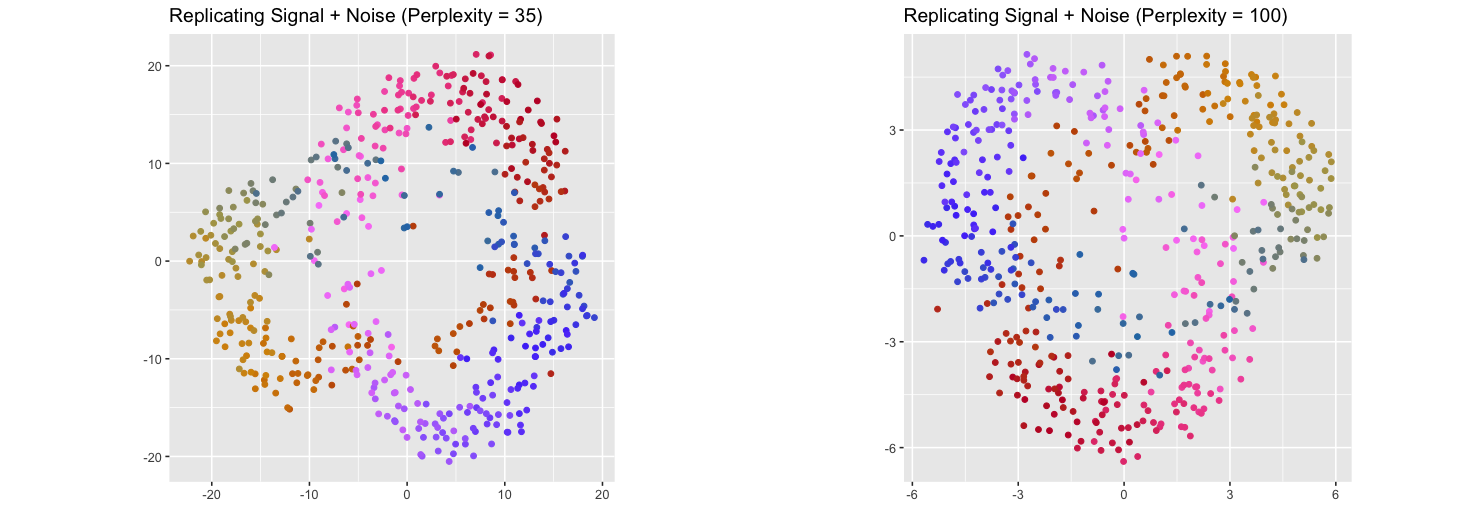
\includegraphics[scale=1.2]{Fig S2}
\caption{{\bf Trustworthiness-maximizing representations for sd = 10 (trefoil).}
Trustworthiness-maximizing t-SNE outputs.}
\end{figure}

\begin{figure}[H]
\centering
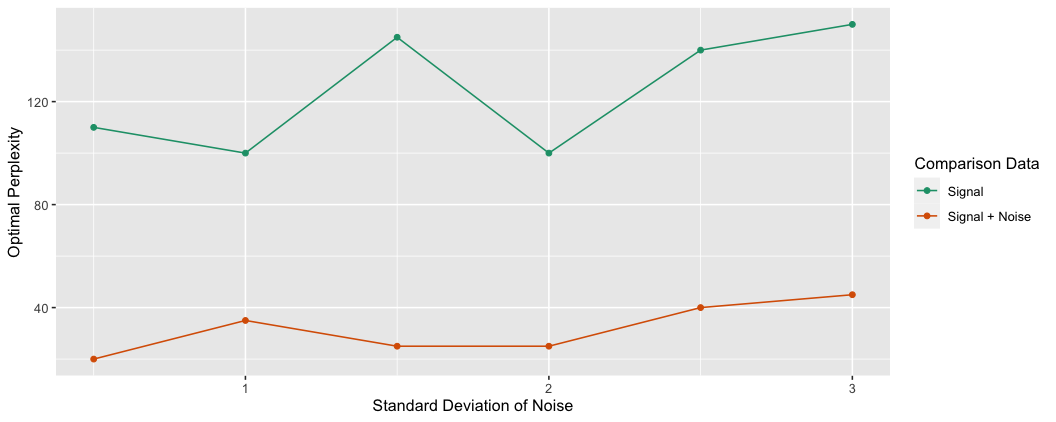
\includegraphics[scale=1.4]{Fig S3}
\caption{{\bf Optimal perplexity (trefoil).}
The experiment was repeated at various levels of noise. For each level of noise, the trustworthiness-maximizing perplexity was recorded when comparing against the original data and the signal. The optimal perplexity was consistently greater when comparing against the signal.}
\end{figure}

\subsection{Mammoth Plots}
For the mammoth example, the signal $Y$ consisted of 500 points in three dimensions. The data was randomly sampled from the mammoth data set used in \cite{understanding DR}. $Z + \epsilon$ was constructed by adding seven superfluous dimensions and isotropic Gaussian noise. Various degrees of noise were tested ($sd = 0.5, 1, 1.5, 2, 2.5, 3$). The first two plots depict Trustworthiness vs. Perplexity and the trustworthiness-maximizing embeddings for the $sd = 1$ case. The third plot shows the trustworthiness-maximizing perplexity for the different degrees of noise.

\begin{figure}[H]
\centering
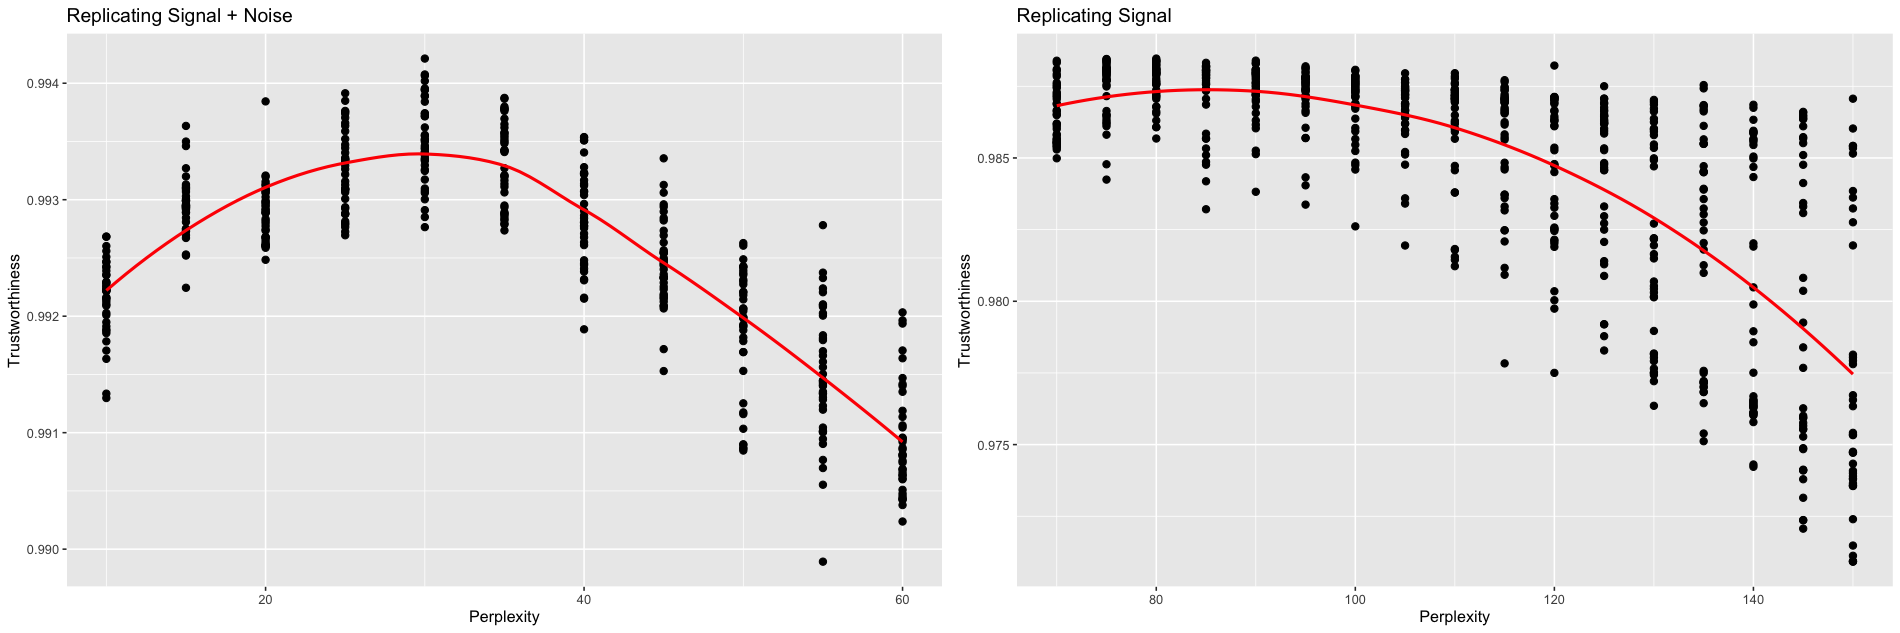
\includegraphics[scale=0.85]{Fig S4}
\caption{{\bf Trustworthiness vs. perplexity for sd = 11 (mammoth).}
t-SNE outputs were calculated with varying perplexities. Local performance was measured via trustworthiness. The trustworthiness-maximizing perplexity was 30 when comparing against the original data, while the trustworthiness-maximizing perplexity was 80 when comparing against just the signal.}
\end{figure}

\begin{figure}[H]
\centering
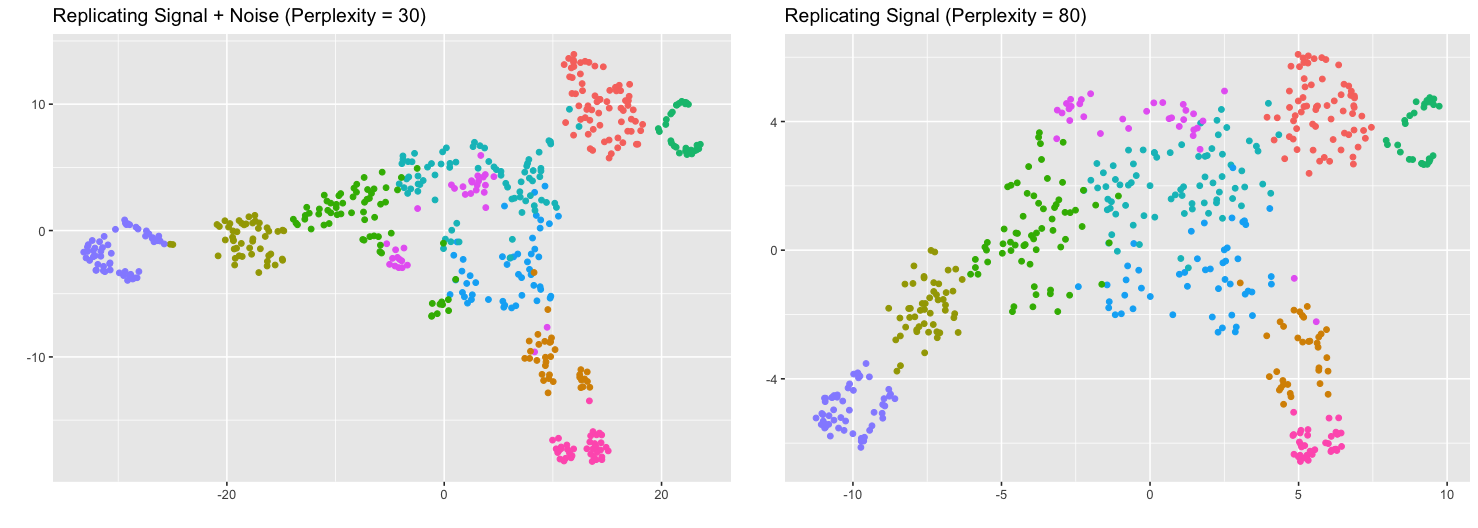
\includegraphics[scale=1.05]{Fig S5}
\caption{{\bf Trustworthiness-maximizing representations (mammoth).}
Trustworthiness-maximizing t-SNE outputs. Labels provided by the authors of the data. The perplexity = 30 representation is more tightly clustered, but incorrectly separated the purple cluster, while the perplexity = 80 representation did not.}
\end{figure}

\begin{figure}[H]
\centering
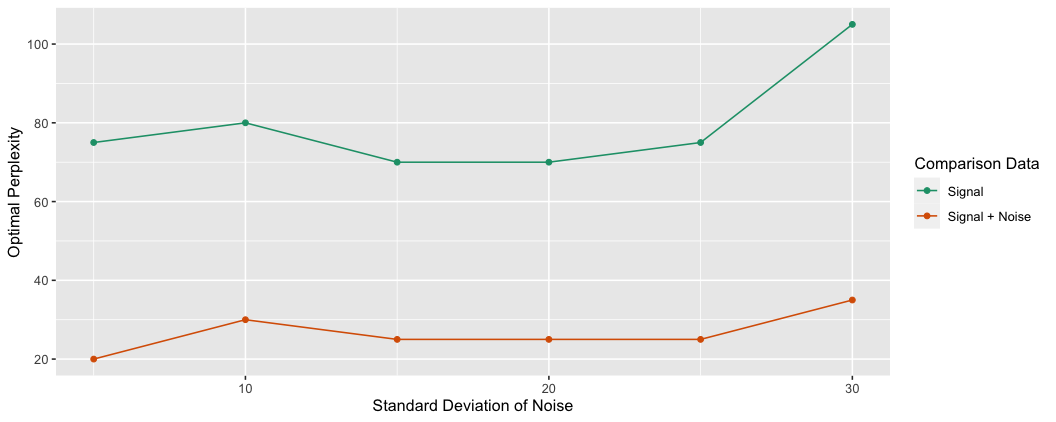
\includegraphics[scale=1.4]{Fig S6}
\caption{{\bf Optimal perplexity (mammoth).}
The experiment was repeated at various levels of noise. For each level of noise, the trustworthiness-maximizing perplexity was recorded when comparing against the original data and the signal. The optimal perplexity was consistently greater when comparing against the signal.}
\end{figure}

\section{Practical Examples}

\subsection{CyTOF Data Set}
The CyTOF data set contained 239,933 observations in 49 dimensions \cite{CyTOF data}. To reduce the computational load, a subset of 5,000 observations was sampled. A log transformation was followed by a PCA pre-processing step to reduce the number of dimensions to 30, which still retained 77\% of the variance in the original data. The processed data set to be studied consisted of 5,000 observations in 30 dimensions. The signal was first taken to be the first five principal components, then the first eight principal components. A hierarchical clustering of the high-dimensional data was computed then projected onto the trustworthiness-maximizing representations.

\begin{figure}[H]
\centering
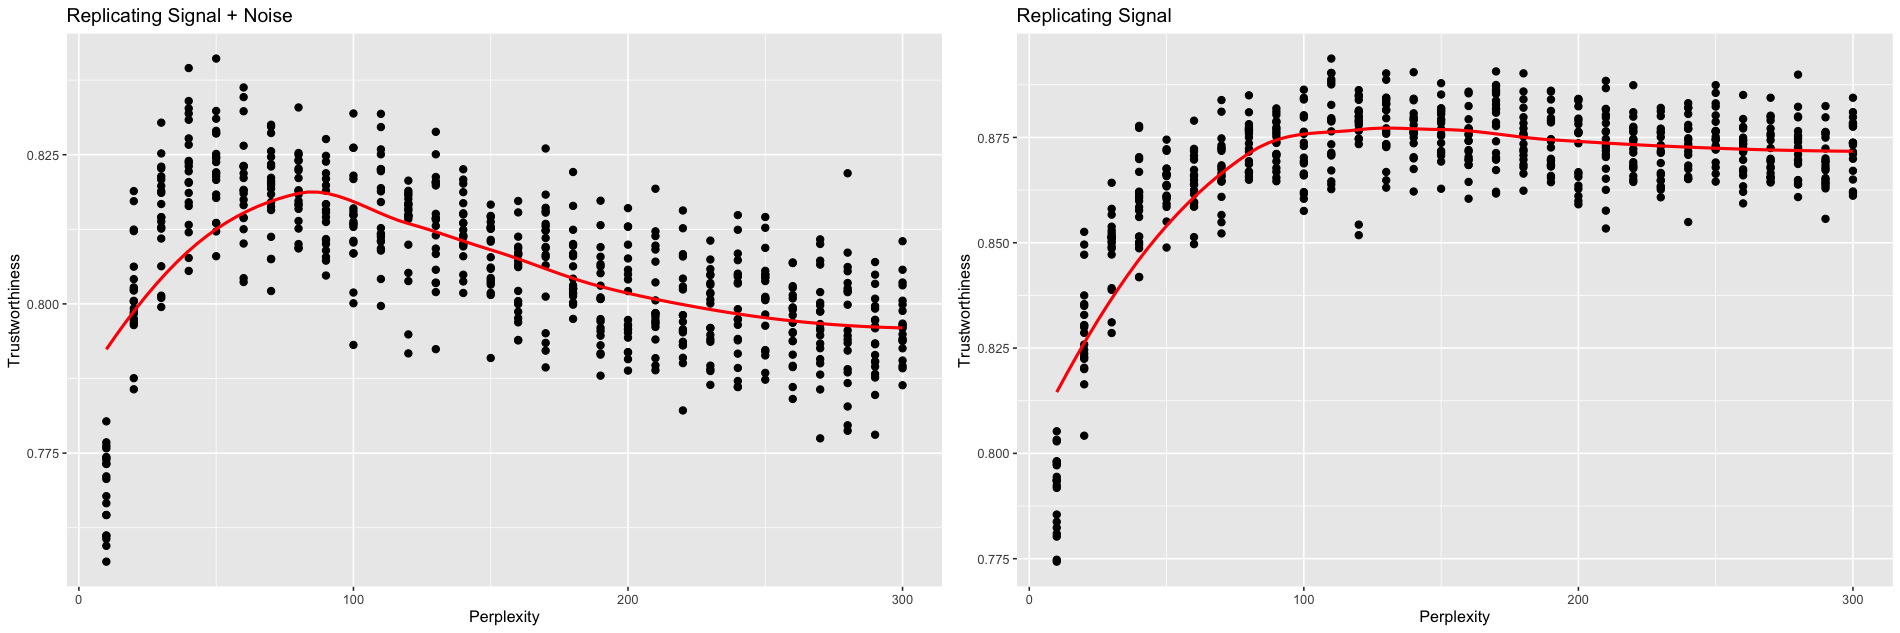
\includegraphics[scale=0.85]{Fig S7}
\caption{{\bf Trustworthiness vs. perplexity for r = 5 (CyTOF).}
t-SNE outputs were calculated with varying perplexities. Local performance was measured via trustworthiness. The trustworthiness-maximizing perplexity was 50 when comparing against the original data, while the trustworthiness-maximizing perplexity was 110 when comparing against just the signal.}
\end{figure}

\begin{figure}[H]
\centering
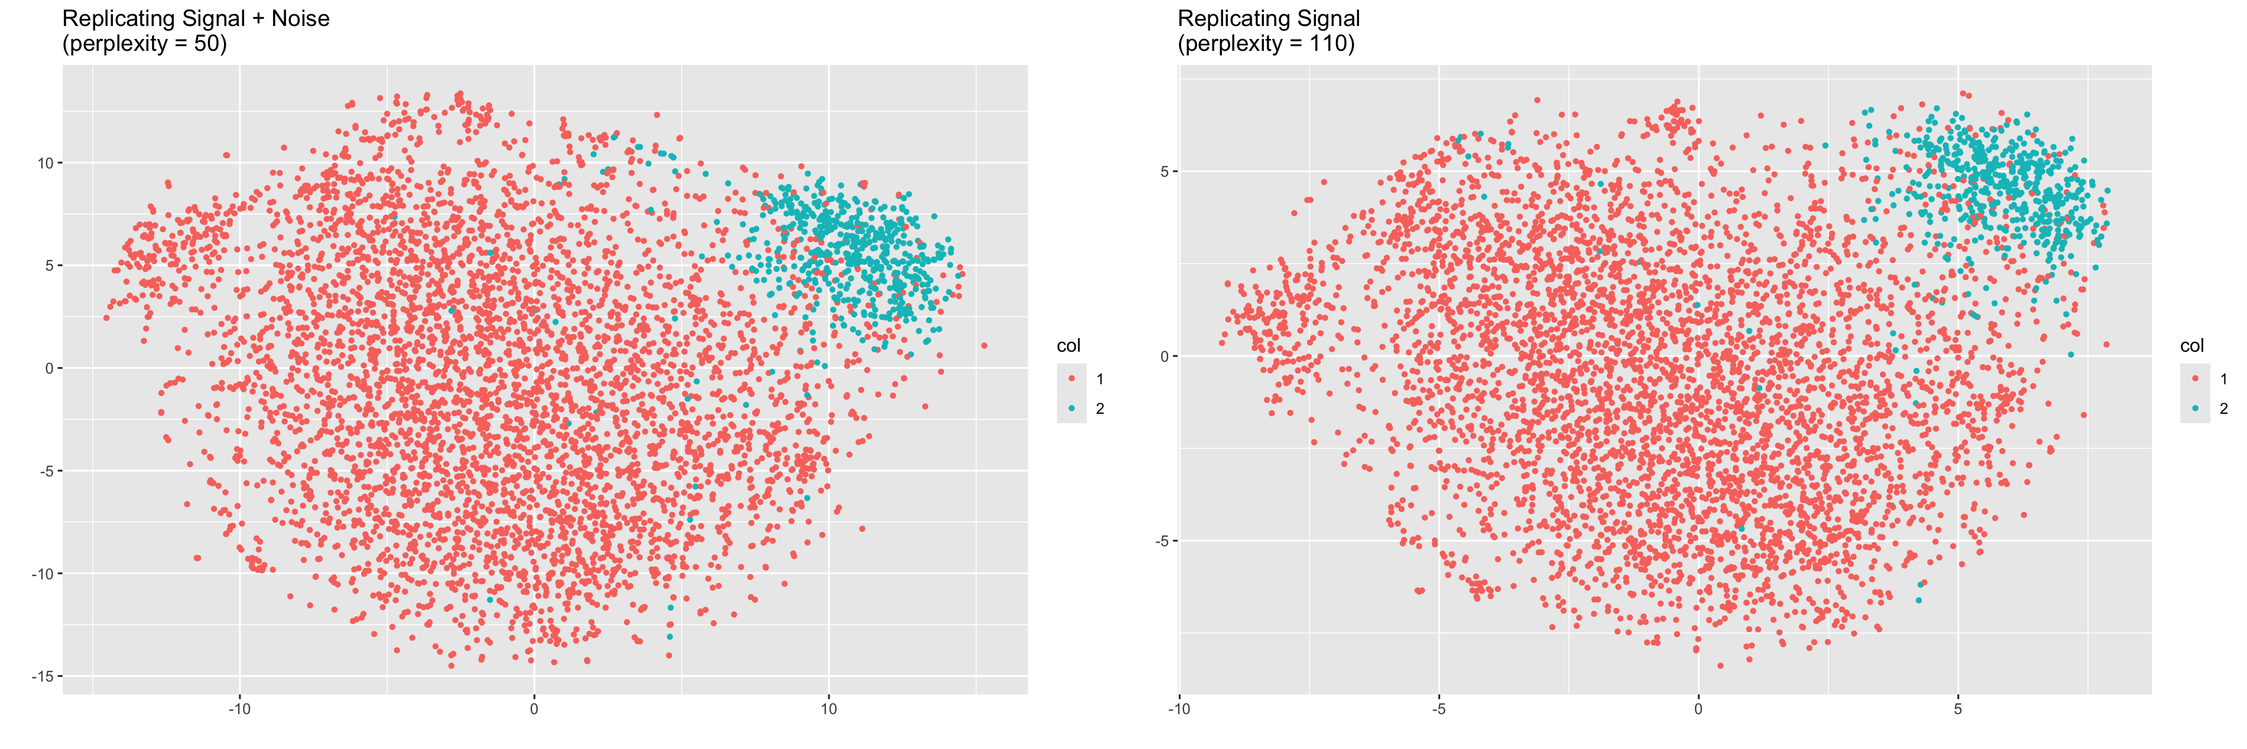
\includegraphics[scale=0.7]{Fig S8}
\caption{{\bf Trustworthiness-maximizing representations for r = 5 (CyTOF).}
Trustworthiness-maximizing t-SNE outputs. Hierarchical clustering applied to high-dimensional data.}
\end{figure}

\begin{figure}[H]
\centering
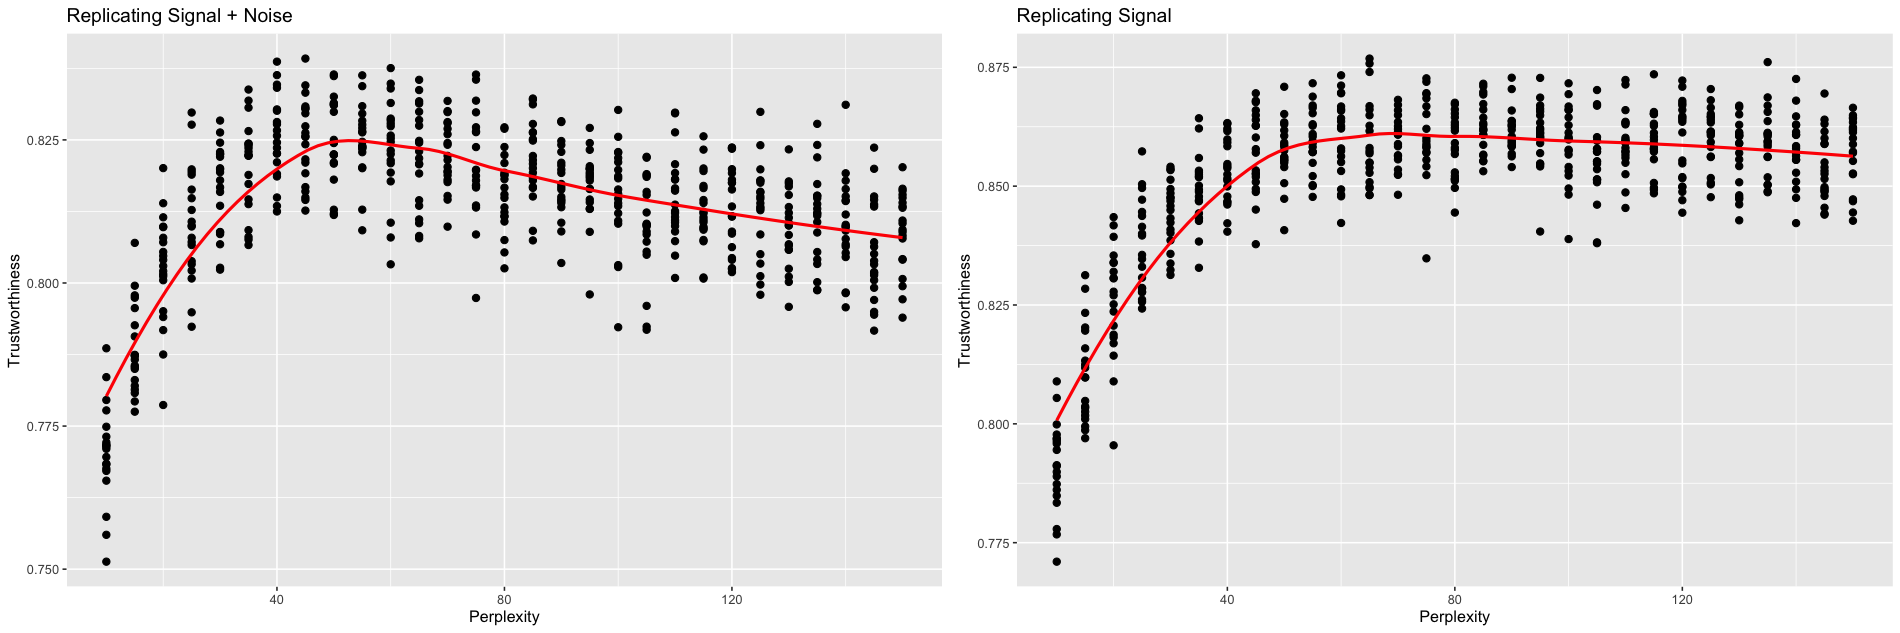
\includegraphics[scale=0.85]{Fig S9}
\caption{{\bf Trustworthiness vs. perplexity for r = 8 (CyTOF).}
t-SNE outputs were calculated with varying perplexities. Local performance was measured via trustworthiness. The trustworthiness-maximizing perplexity was 45 when comparing against the original data, while the trustworthiness-maximizing perplexity was 65 when comparing against just the signal.}
\end{figure}

\begin{figure}[H]
\centering
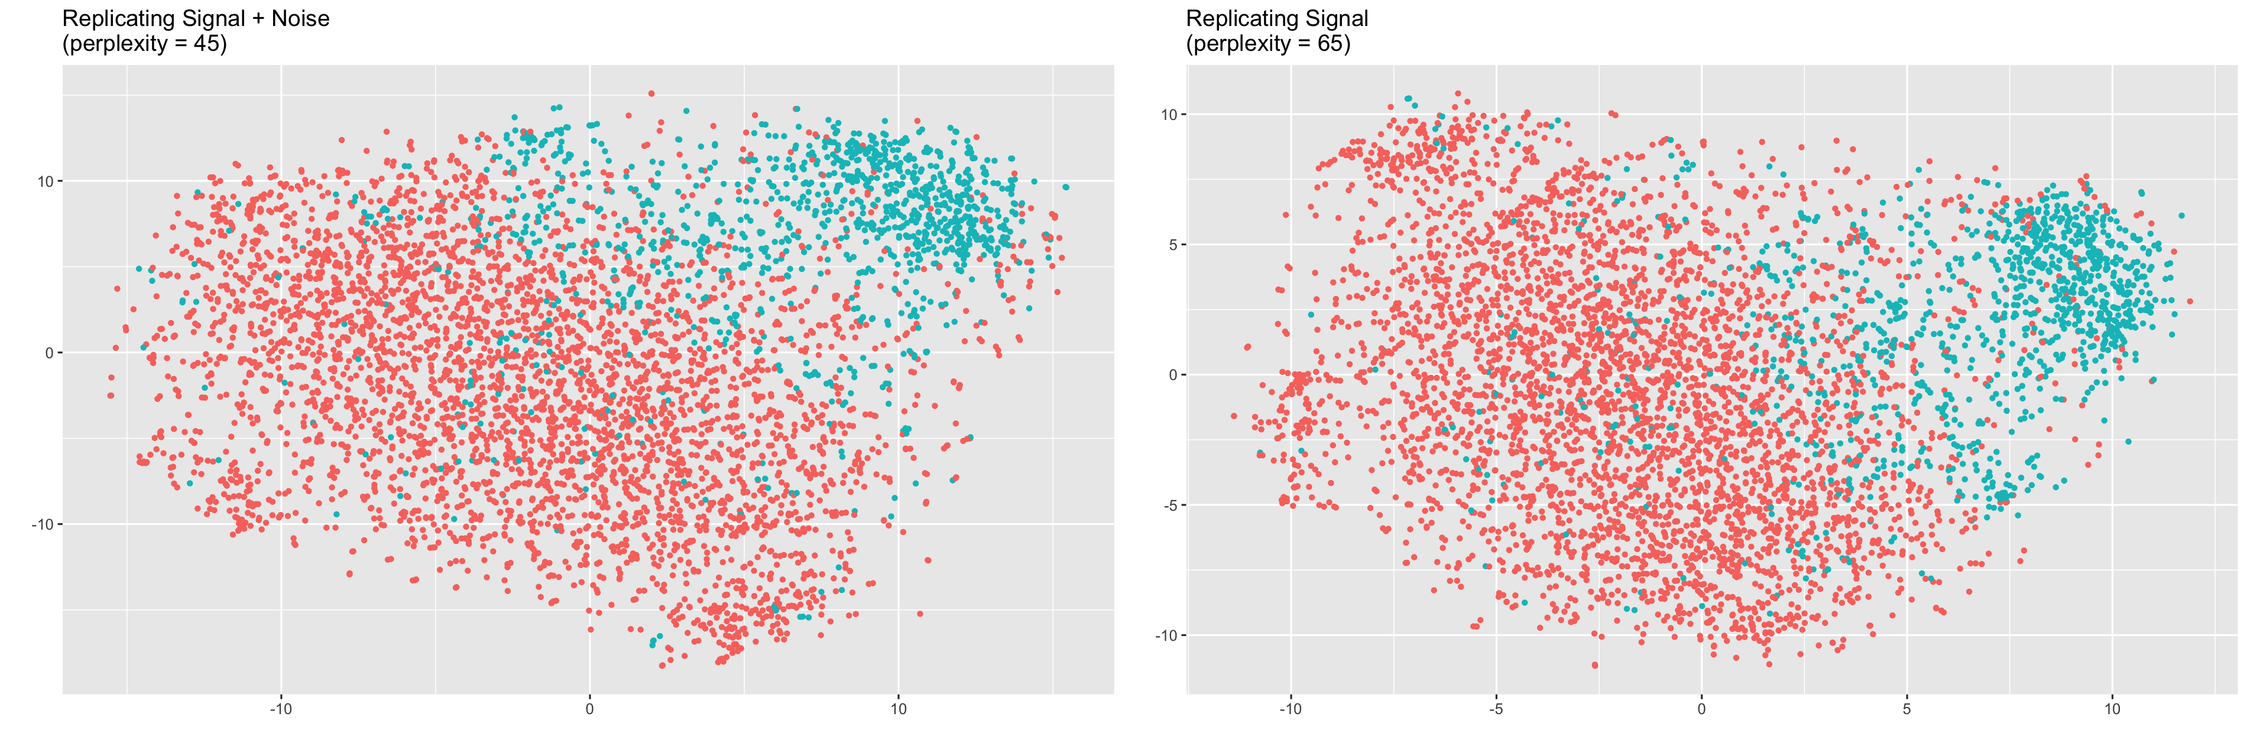
\includegraphics[scale=0.7]{Fig S10}
\caption{{\bf Trustworthiness-maximizing representations for r = 8 (CyTOF).}
Trustworthiness-maximizing t-SNE outputs. Hierarchical clustering applied to high-dimensional data.}
\end{figure}

\subsection{Microbiome Data Set}
\cite{enterotype data} compares the faecal microbial communities from 22 subjects using complete shotgun DNA sequencing. The original data contained 280 samples and 553 genera. To deal with a large number of near-zero readings, columns containing a large proportion of values less than $10^{-6}$ (60\% or more) were removed. This reduced the dimension to 66. A PCA pre-processing was used to center and re-scale the data. The signal was first taken to be the first five principal components, then the first eight principal components. A k-means clustering of the high-dimensional data was computed then projected onto the trustworthiness-maximizing representations.

\begin{figure}[H]
\centering
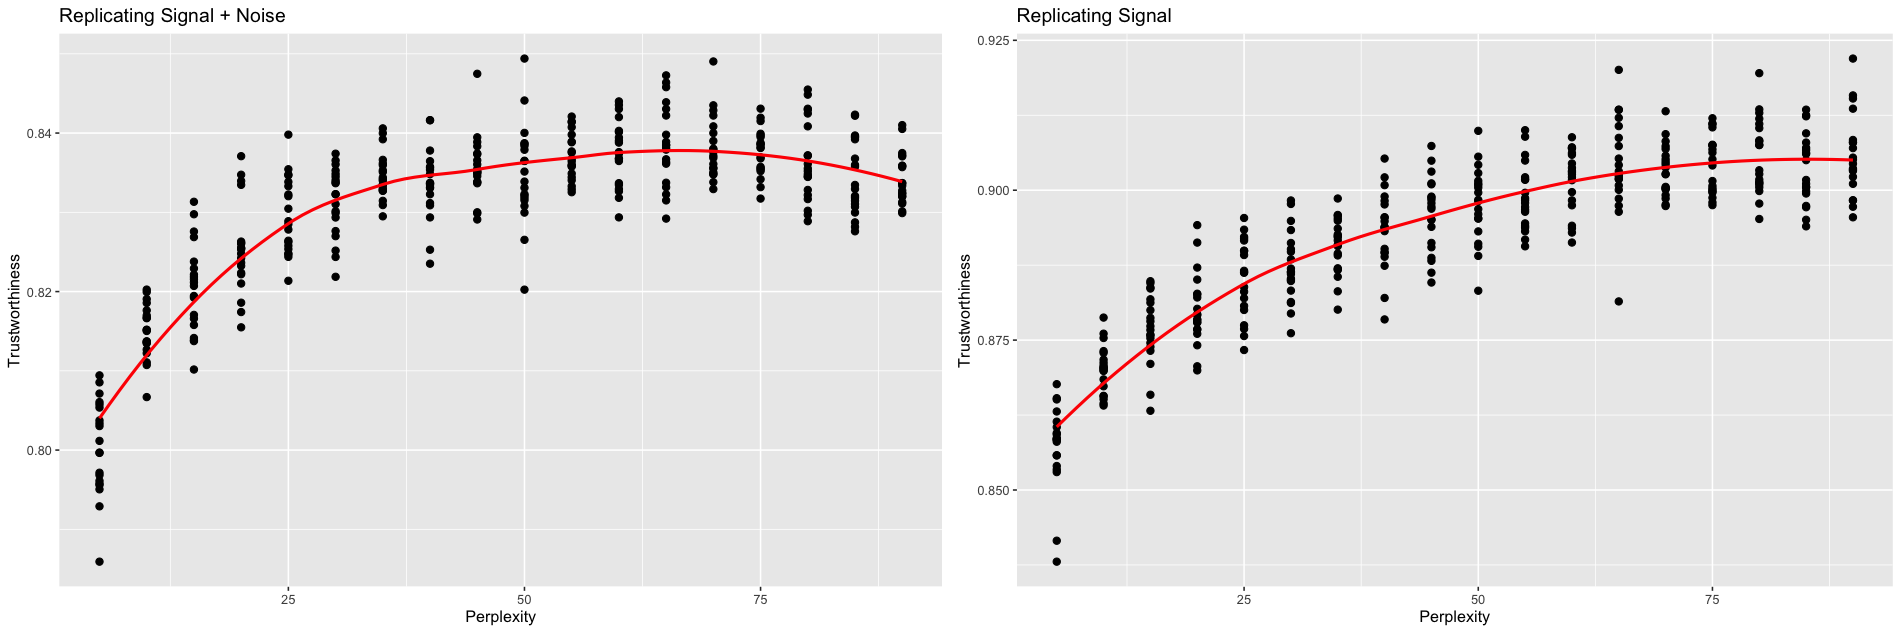
\includegraphics[scale=0.85]{Fig S11}
\caption{{\bf Trustworthiness vs. perplexity for r = 5 (microbiome).}
t-SNE outputs were calculated with varying perplexities. Local performance was measured via trustworthiness. The trustworthiness-maximizing perplexity was 50 when comparing against the original data, while the trustworthiness-maximizing perplexity was 90 when comparing against just the signal.}
\end{figure}

\begin{figure}[H]
\centering
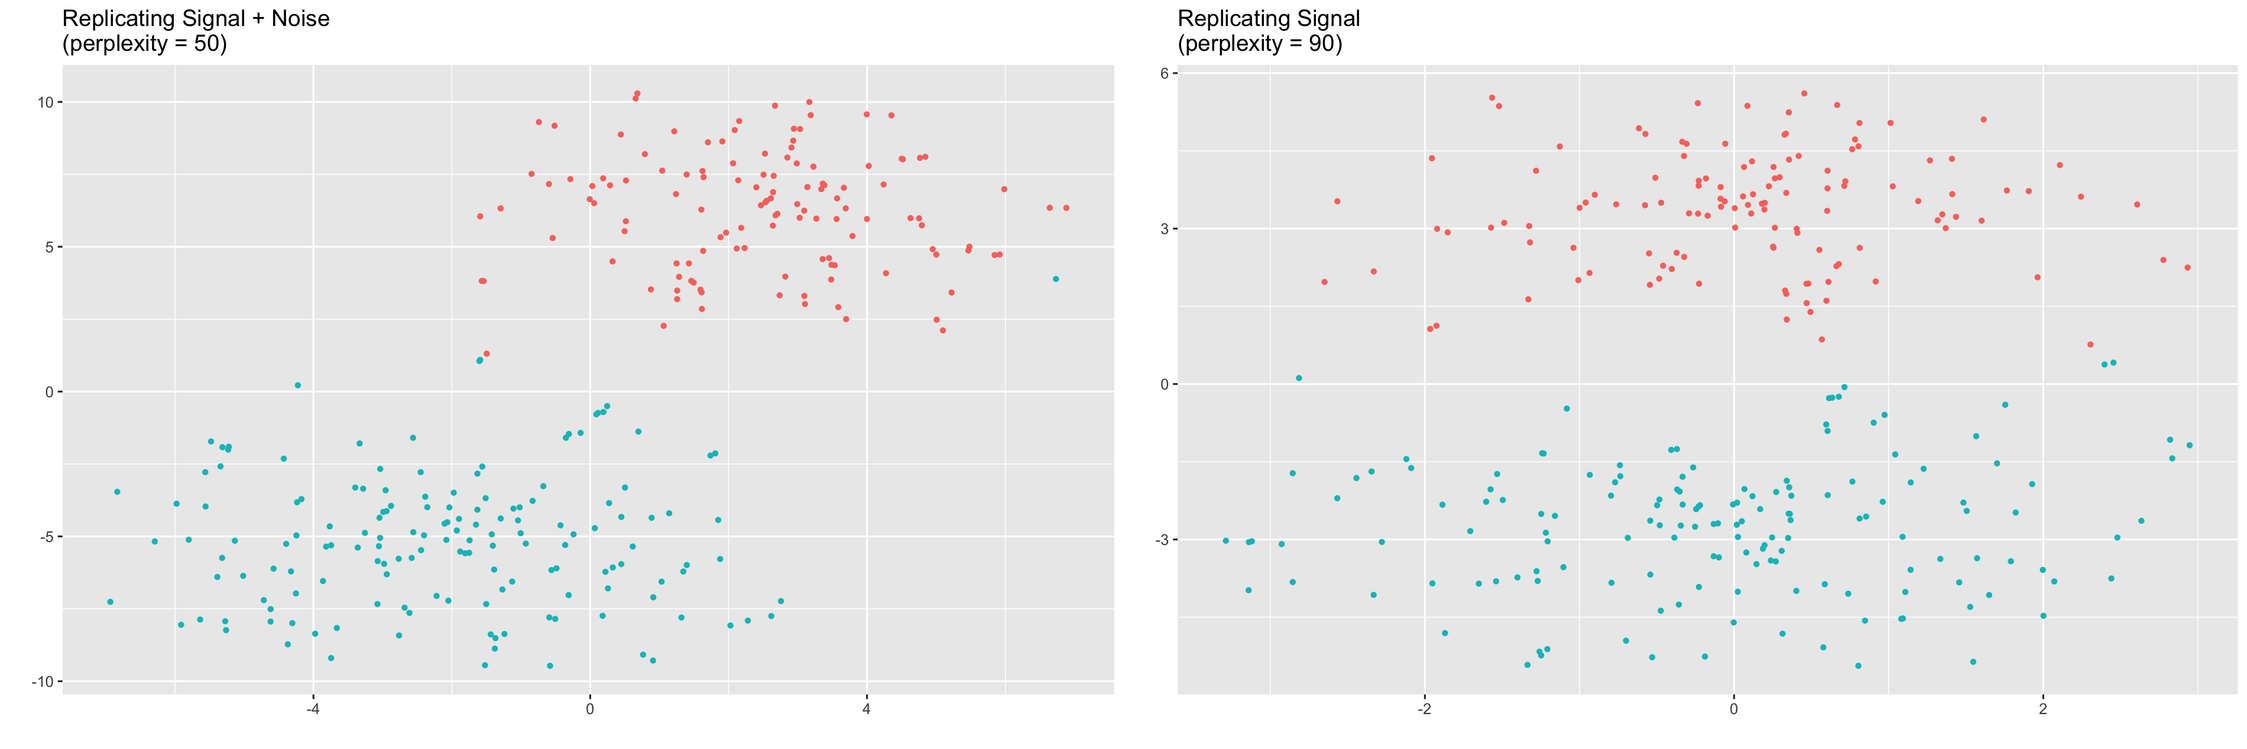
\includegraphics[scale=0.7]{Fig S12}
\caption{{\bf Trustworthiness-maximizing representations for r = 5 (microbiome).}
Trustworthiness-maximizing t-SNE outputs. K-means clustering applied to high-dimensional data.}
\end{figure}

\begin{figure}[H]
\centering
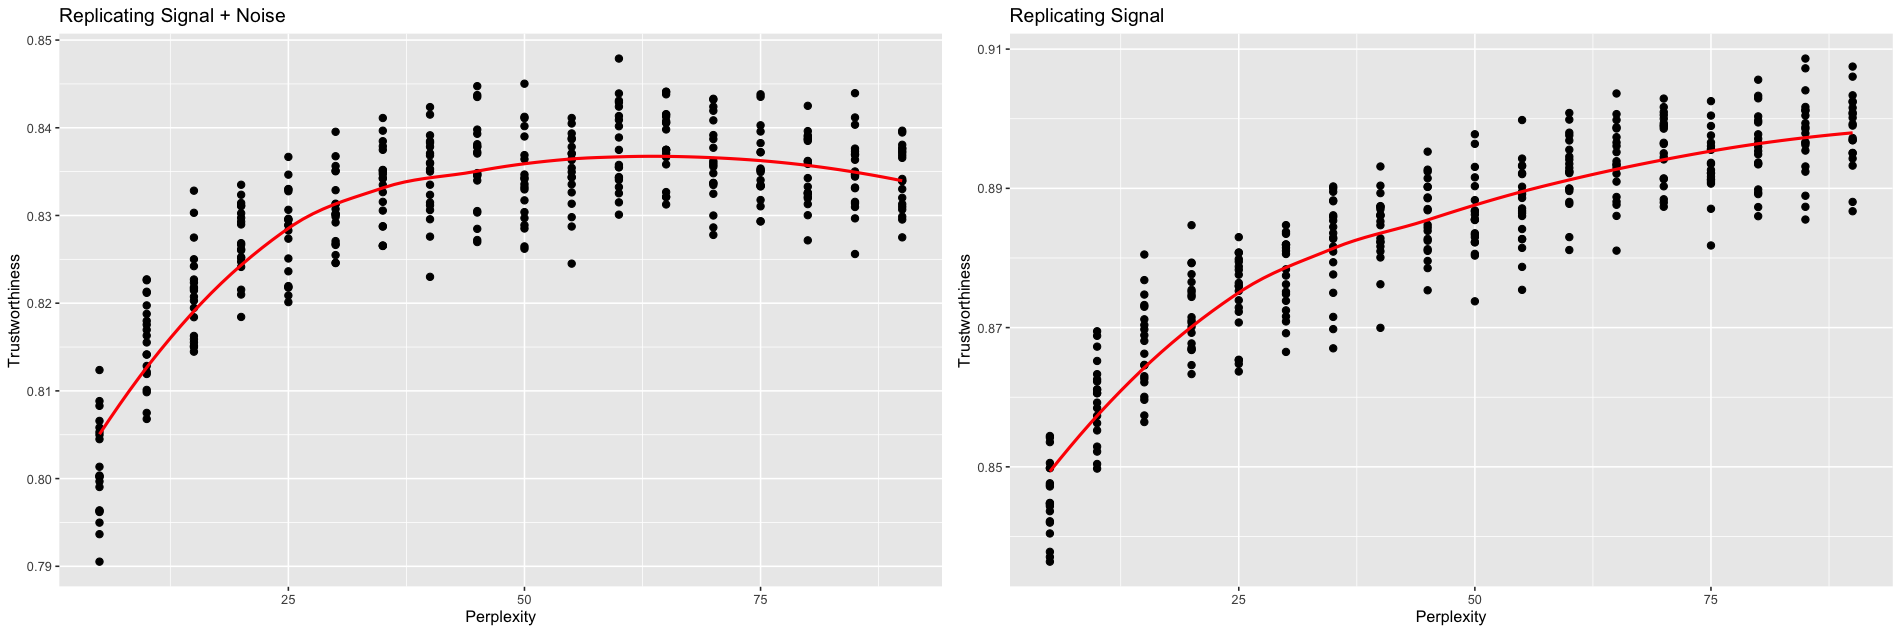
\includegraphics[scale=0.85]{Fig S13}
\caption{{\bf Trustworthiness vs. perplexity for r = 8 (microbiome).}
t-SNE outputs were calculated with varying perplexities. Local performance was measured via trustworthiness. The trustworthiness-maximizing perplexity was 60 when comparing against the original data, while the trustworthiness-maximizing perplexity was 85 when comparing against just the signal.}
\end{figure}

\begin{figure}[H]
\centering
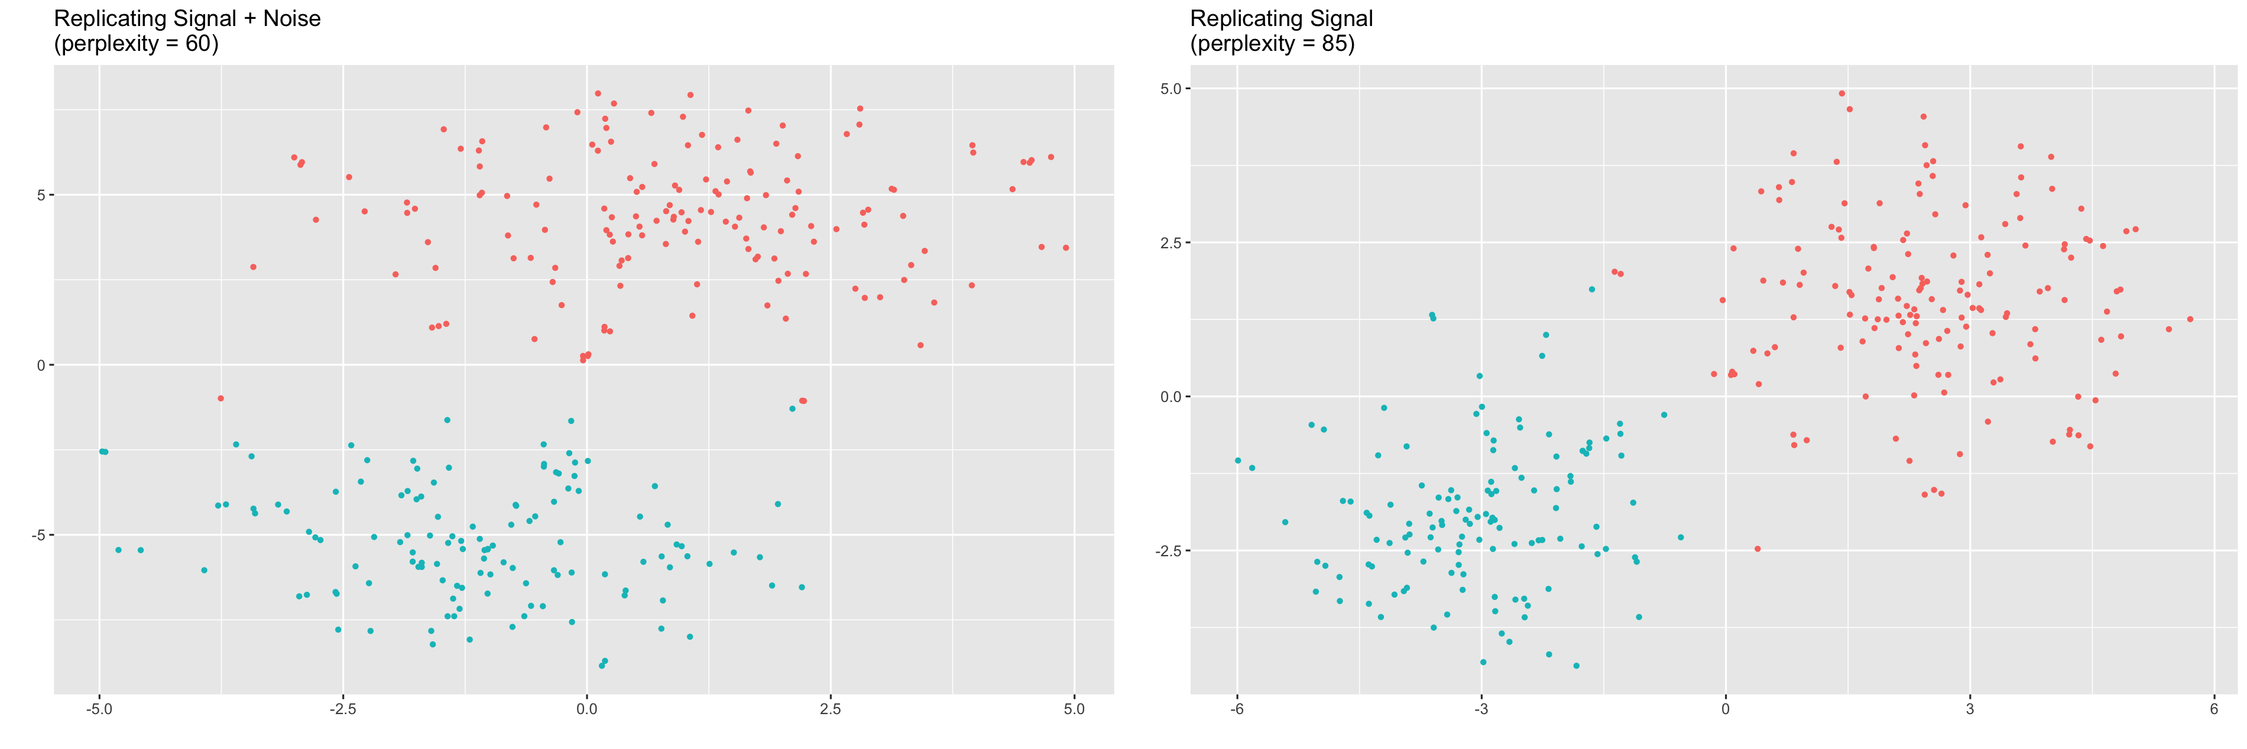
\includegraphics[scale=0.7]{Fig S14}
\caption{{\bf Trustworthiness-maximizing representations for r = 8 (microbiome).}
Trustworthiness-maximizing t-SNE outputs. K-means clustering applied to high-dimensional data.}
\end{figure}

\section{PBMC Data Set}
Further examination of the dendritic cells shows that they belong to multiple clusters. To determine the number of clusters, we employ average silhouette width and the gap statistic.

\begin{figure}[H]
\centering
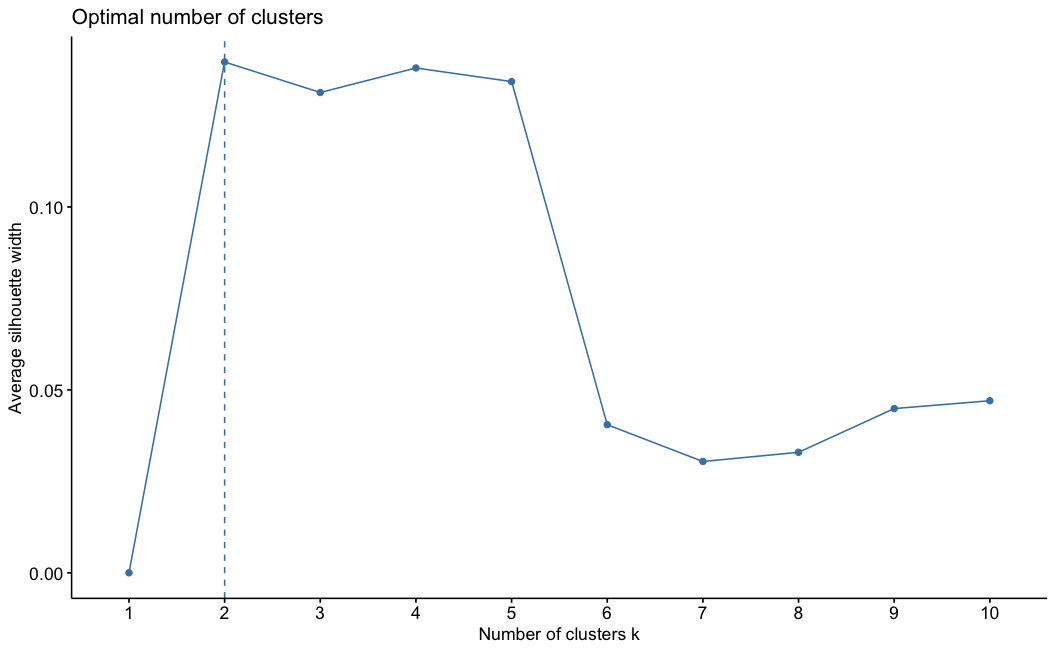
\includegraphics[scale=0.33]{Fig S15}
\caption{{\bf Average silhouette width for dendritic cells.}
The average silhouette width suggests two clusters are appropriate.}
\end{figure}

\begin{figure}[H]
\centering
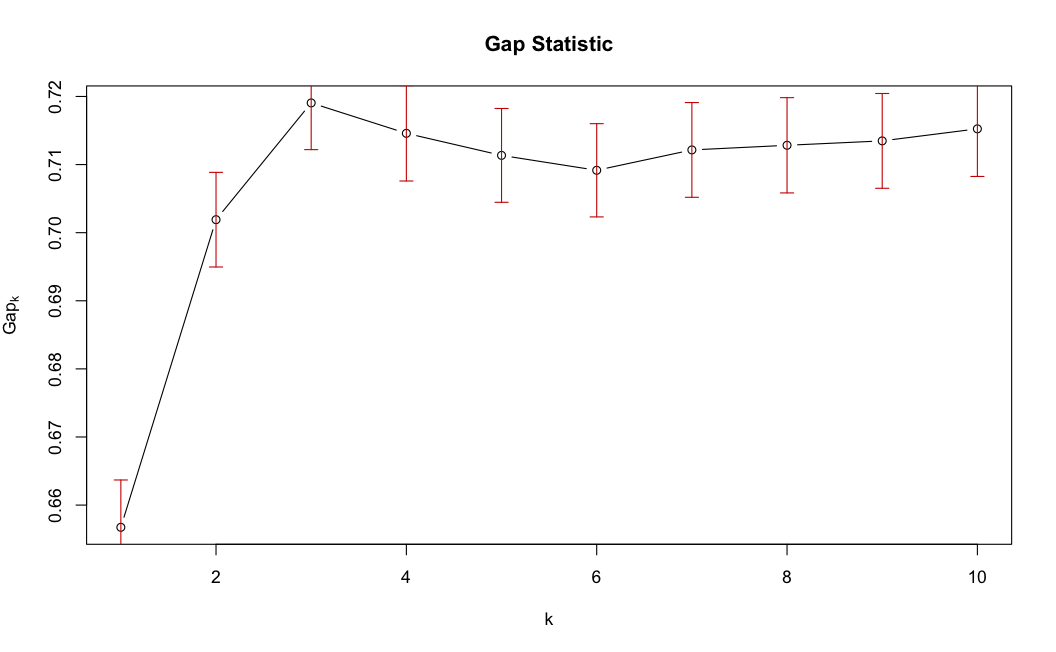
\includegraphics[scale=0.33]{Fig S16}
\caption{{\bf Gap statistic for dendritic cells.}
The gap statistic suggests three clusters are appropriate.}
\end{figure}

\newpage
\bibliographystyle{abbrvnat}
\bibliography{reference}

\begin{thebibliography}{10}

\bibitem{t-SNE example}
Amir ED, Davis KL, Tadmor MD, Simonds EF, Levine JH, Bendall SC, et al.
\newblock viSNE enables visualization of high dimensional single-cell data and reveals phenotypic heterogeneity of leukemia.
\newblock Nat Biotechnology. 2013 May 19;31:545-52.

\bibitem{SVD example}
Alter O, Brown PO, Botstein D.
\newblock Singular value decomposition for genome-wide expression data processing and modeling.
\newblock PNAS. 2000 Aug 29;97(18):10101-6.

\bibitem{PHATE}
Moon KR, van Dijk D, Wang Z, Gigante S, Burkhardt DB, Chen WS, et al.
\newblock Visualizing structure and transitions in high-dimensional biological data.
\newblock Nat Biotechnology. 2019 Dec 3;37:1482-92.

\bibitem{t-SNE}
van der Maaten L, Hinton G.
\newblock Visualizing data using t-SNE.
\newblock JLMR. 2008 Nov 8;9:2579-605.

\bibitem{umap}
McInnes L, Healy J, Melville J.
\newblock UMAP: Uniform Manifold Approximation and Projection for dimension reduction.
\newblock arXiv:1802.03426v3 [Preprint]. 2020. Available from https://arxiv.org/abs/1802.03426.

\bibitem{UMAP example}
Becht E, McInnes L, Healy J, Dutertre CA, Kwok IWH, Ng LG, et al.
\newblock Dimensionality reduction for visualizing single-cell data using UMAP.
\newblock Nat Biotechnology. 2019 Dec 3;37:28-44.

\bibitem{t-SNE/UMAP example}
Kobak D, Linderman GC.
\newblock Initialization is critical for preserving global data structure in both t-SNE and UMAP.
\newblock Nat Biotechnology. 2021 Feb 1;39:156-7.

\bibitem{perplexity-free t-SNE}
Crecchi F, de Bodt C, Verleysen M, Lee JA, Bacciu D.
\newblock Perplexity-free parametric t-SNE.
\newblock arXiv:2010.01359v1 [Preprint]. 2020. Available from https://arxiv.org/abs/2010.01359.

\bibitem{evaluation of DR transcriptomics}
Huang H, Wang Y, Rudin C, Browne EP.
\newblock Towards a comprehensive evaluation of dimension reduction methods for transcriptomic data visualization.
\newblock Commun Biol. 2022 July 19;5(1):719.

\bibitem{t-SNE cell}
Kobak D, Berens P.
\newblock The art of using t-SNE for single-cell transcriptomics.
\newblock Nat Communications. 2019 Nov 28;10:5416.

\bibitem{perplexity vs kl}
Cao Y, Wang L. 
\newblock Automatic selection of t-SNE perplexity.
\newblock arXiv:1708.03229.v1 [Preprint]. 2017. Available from https://arxiv.org/abs/1708.03229.

\bibitem{diffusion maps}
Coifman RR, Lagon S.
\newblock Diffusion maps.
\newblock Applied and Computational Harmonic Analysis. 2006 July;21(1):5-30.

\bibitem{Distill}
Wattenberg M, Vi\'egas F, Johnson I.
\newblock How to Use t-SNE Effectively.
\newblock Distill. 2016. Available from https://distill.pub/2016/misread-tsne/.

\bibitem{understanding UMAP}
Coenen A, Pearce A for Google PAIR.
\newblock Understanding UMAP.
\newblock Available from https://pair-code.github.io/understanding-umap/.

\bibitem{large DR unreliable}
Chari T, Pachter L.
\newblock The specious art of single-cell genomics.
\newblock PLoS Computational Biology. 2017 Aug 17;19(8): e1011288.

\bibitem{quantitative survey}
Espadoto M, Martins RM, Kerren A, Hirata NST, Telea AC.
\newblock Towards a quantitative survey of dimension reduction techniques.
\newblock  IEEE Transactions on Visualization and Computer Graphics. 2021 Mar;27(3):2153-73.

\bibitem{trustworthiness}
Venna J, Kaski S.
\newblock Visualizing gene interaction graphs with local multidimensional scaling.
\newblock ESANN. 2006 Apr 26-28.

\bibitem{understanding DR}
Wang Y, Huang H, Rudin C, Shaposhnik Y.
\newblock Understanding how dimension reduction tools work: An empirical approach to deciphering t-SNE, UMAP, TriMap, and PaCMAP for data visualization.
\newblock JMLR. 2021;22:1-73.

\bibitem{Rtsne}
Krijthe JH.
\newblock Rtsne: T-Distributed Stochastic Neighbor Embedding using a Barnes-Hut implementation.
\newblock Available from https://github.com/jkrijthe/Rtsne.

\bibitem{scRNA data}
Tung PY, Blischak JD, Hsiao CJ, Knowles DA, Burnett JE, Pritchard JK, et al.
\newblock Batch effects and the effective design of single-cell gene expression studies.
\newblock Scientific Reports. 2017 Jan 3;7:39921.

\bibitem{CyTOF data}
Strauss-Albee DM, Fukuyama J, Liang EC, Yao Y, Jarrell JA, Drake AL, et al.
\newblock Human NK cell repertoire diversity reflects immune experience and correlates with viral susceptibility.
\newblock Science Translational Medicine. 2015 July 22;7(297):297.

\bibitem{enterotype data}
Arumugam M, Raes J, Pelletier E, Paslier DL, Yamada T, Mende DR, et al.
\newblock Enterotypes of the human gut microbiome.
\newblock Nature. 2011 Apr 20;473:174-80.

\bibitem{parallel analysis}
Horn JL.
\newblock A rationale and test for the number of factors in factor analysis.
\newblock Psychometrika. 1965 June;30:179-85.

\bibitem{subsample t-SNE}
Skrodzki M, Chaves-de-Plaza N, Hildebrandt K, H\"ollt T, Eisemann E.
\newblock Tuning the perplexity for and computing sampling-based t-SNE embeddings.
\newblock arXiv:2308.15513 [Preprint]. 2023 Aug 29. Available from https://arxiv.org/abs/2308.15513.

\bibitem{BPCells data}
Cell Ranger ARC 2.0.0.
\newblock PBMC from a healthy donor - granulocytes removed through cell sorting (3k).
\newblock 10x Genomics. 2021 May 5.

\bibitem{BPCells tutorial}
Parks B.
\newblock BPCells: single cell counts matrices to PCA.
\newblock 2024. Available from https://bnprks.github.io/BPCells.

\bibitem{noise in single-cell data}
Chu SK, Zhao S, Shyr Y, and Liu Q.
\newblock Comprehensive evaluation of noise reduction methods for single-cell RNA sequencing data.
\newblock Briefings in Bioinformatics. 2022 Mar 10;23(2).

\bibitem{TriMap}
Amid E, Warmuth MK. 
\newblock TriMap: Large-scale dimensionality reduction using triplets. 
\newblock arXiv:1910.00204.v2 [Preprint]. 2022 Mar 26. Available from https://arxiv.org/abs/2308.15513.

\bibitem{rank-based criteria}
Lee JA, Verleysen M.
\newblock Quality assessment of dimensionality reduction: Rank-based criteria.
\newblock Neurocomputing. 2009 Mar;72(7-9):1431-43.

\bibitem{precision score}
Schreck T, von Landesberger T, Bremm S.
\newblock Techniques for precision-based visual analysis of projected data.
\newblock Sage. 2012 Jan 1;9(3).

\end{thebibliography}

\end{document}
